Durch die optischen Besonderheiten von spiegelnd glänzenden Oberflächen treten solche in der Industrie an vielen Stellen auf.
Speziell in der Automobilindustrie werden täglich große Karosserieflächen glänzend lackiert.
Alleine in Deutschland wurden in den Jahren von 1990 bis 2021 im Durchschnitt ungefähr 5 Millionen Personenkraftwagen pro Jahr produziert. \cite{statistaPKW}
Ein großer Teil der Fahrzeuge erhalten nach der Lackierung eine spiegelnde Oberfläche.
Solche Oberflächen müssen durch besondere Verfahren auf Defekte überprüft werden.
Dabei sorgen spekulare Reflexionen dafür, dass die Oberflächen nicht direkt, sondern über ihre Spiegelbilder der Umgebung betrachtet werden. %TODO Beispielbilder?

\p
Die riesige Menge an Oberflächen macht es für die Qualitätssicherung unumgänglich die Prüfung durch automatisierte Prozesse zu integrieren.
Dabei stoßen die üblichen Verfahren der industriellen Bildverarbeitung auf ihre Grenzen, sodass neue Methoden eingeführt werden müssen.
Diese speziellen Anwendungen erfordern den Einsatz von deflektometrischen Prüfaufbauten.
In der Industrie sind solche Verfahren schon seit Längerem zur Analyse der Topographie von spiegelnden Freiformflächen etabliert.
Deflektometrische Verfahren funktionieren nach einem ähnlichen Prinzip, wie auch die Inspektion von spiegelnden Oberflächen durch Menschen.
Das wissenschaftliche Gebiet der Deflektometrie ist auch heute noch Thema für viele Forschungsarbeiten und wird stetig weiterentwickelt.

\p
Im Rahmen der Arbeit werden spekular reflektierende Objektoberflächen unter Projektion von bekannten Mustern durch eine Kamera aufgenommen, anschließend analysiert und auf Defekte überprüft.
Welche Informationen können aus der Beobachtung von Spiegelbildern gewonnen werden?
Wie sehen allgemein anwendbare Methoden aus, um spiegelnde Oberflächen erfolgreich zu bewerten?
Das Ziel der Arbeit ist es, diese Fragen zu erforschen und aufzuklären.
Des Weiteren sollen ein Aufbau, die Ansteuerung von Beleuchtung und Kamera und die notwendige Auswertung des Bildmaterials entwickelt werden, durch welche eine Erkennung von Oberflächendefekten ermöglicht wird.
Die Umsetzung soll dabei in Form einer Softwareerweiterung für NeuroCheck erfolgen, eines sogenannten \textit{Plug-ins}.

\p
Während der Arbeit soll außerdem ein bestimmter Sonderfall genauer betrachtet werden - transparente Prüfobjekte.
Die Problematik ist dabei, dass man ohne Weiteres kein sichtbares Muster auf die Oberfläche projizieren kann.
Dafür gibt es verschiedene Lösungsansätze wie z. B. die Auftragung einer undurchsichtigen Beschichtung.
Eine andere Möglichkeit ist eine Veränderung in der Beleuchtungskomponente.
Anstatt ein Muster auf das Objekt zu projizieren, kann man eine Durchlichtbeleuchtung nutzen.
Das heißt, dass man auf einem Bildschirm unter dem transparenten Prüfobjekt verschiedene Muster anzeigt.

\p
Durch die aufgenommenen Muster können Aussagen über die Oberflächenbeschaffenheit getroffen werden.
Abhängig von den verwendeten Mustern und der Auswertung sollen damit bestimmte Fehlstellen kenntlich gemacht werden.
Als Fehlstellen gelten Verformungen und Oberflächendefekte wie z. B. Dellen, Kratzer oder matte Stellen.
%TODO Weiteres schreiben im Bezug auf die nachfolgende Arbeit (vermutlich eher gegen Ende)
%Zur Detektion dieser Defekte kann man verschiedene deflektometrische Verfahren einsetzen.
%Die Verfahren können verschiedene Ergebnisse liefern, abhängig davon sind eventuell aus den Ergebnissen weitere Verarbeitungen und Auswertungen nötig.
%Im Rahmen des Projektes werden speziell die deflektometrischen Verfahren betrachtet, welche für eine Vielzahl von Anwendungen genutzt werden können.
%Nachfolgende Verarbeitungen, z. B. Detektion von Zeichen und Kratzern, werden im Rahmen des Projekts und der Bachelor-Arbeit nicht genauer behandelt.

%Deflektometrie
{
	\FloatBarrier
    \section{Einführung in die Deflektometrie}
    \label{sec:deflektometrie}
    \begin{Definition}{Deflektometrie}{def:deflektometrie}
	Die \textit{Deflektometrie} bezeichnet allgemein alle Methoden zur berührungslosen optischen Erfassung von Gestaltinformationen spiegelnder Oberflächen durch automatische Auswertung von Spiegelbildern bekannter Szenen. \cite{fraunhofer}
\end{Definition}

\noindent
Diese Definition öffnet ein großes Gebiet für verschiedene Verfahren und Anwendungen.
Die Verfahren der Deflektometrie sind auch heute noch Themen für viele Forschungsarbeiten.
Im Folgenden soll dabei auf den Stand der Technik der Deflektometrie eingegangen werden.
%TODO Vielleicht noch mehr zur Deflektometrie?

%Rekonstruktion von spiegelnden Oberflächen
{
	\FloatBarrier
    \subsection{Rekonstruktion von spiegelnden Oberflächen}
    \label{sub:rekonstruktion}
    Bei der Recherche zur allgemeinen Deflektometrie fällt auf, dass das Hauptforschungsgebiet der gegenwärtigen Deflektometrie die Generierung von dreidimensionalen Modellen von spiegelnden Objektoberflächen ist.
Der Aufbau eines solchen Anwendungsfalls sieht eine Beleuchtungseinheit (z. B. einen Bildschirm), ein Sensor (z. B. eine Kamera) und ein zu untersuchendes Objekt vor.

\begin{figure}[H]
	\centering
	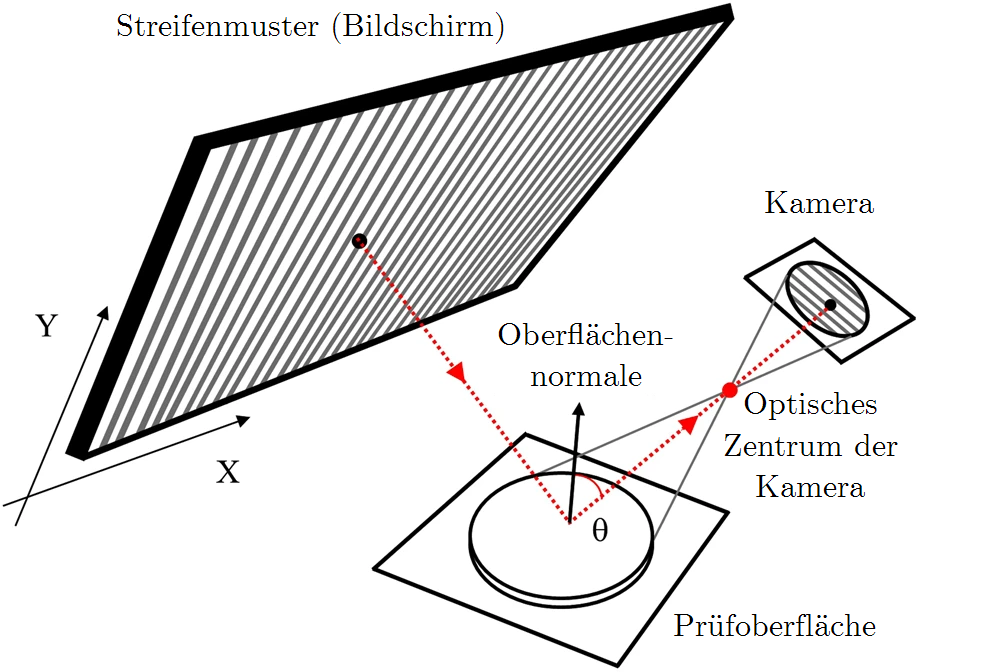
\includegraphics[width=0.8\textwidth]{01_einfuehrung/deflektometrie/rekonstruktion/figures/nature-articel-nr1}
	\caption[Aufbau einer Deflektometrie-Prüfstation]{Aufbau einer Deflektometrie-Prüfstation. \textit{in Anlehnung an} \cite{aufbau}}
	\label{img:aufbau}
\end{figure}

\noindent
Wie in Abbildung \ref{img:aufbau} angedeutet, wird ein Muster auf ein Prüfobjekt projiziert und anschließend von einer Kamera aufgenommen.
Für dieses Verfahren werden zur Projektion üblicherweise Streifenmuster ge\-wählt, deren Grauwertverläufe in ihren Ausbreitungsrichtungen einer Sinus-Funktion entsprechen.
Das grundlegende Prinzip basiert darauf, dass jeder Punkt des Objekts dem richtigen Punkt auf dem Bildschirm zugeordnet wird.
Dabei ordnet man jedem Pixel des projizierten Musters, das man über die Kamera aufnimmt, sein zugehöriges Pixel des erzeugten Musters auf dem Bildschirm zu.
Der Vorteil bei sinusförmigen Streifenmustern ist, dass man für die Punkte des Objekts jeweils den Phasenwinkel im sinusförmigen Muster berechnen kann.
Dies erleichtert die Zuordnung von Kamera- und Bildschirmpunkten.
Durch diese Zuordnung von Kamera- und Bildschirmpunkten lassen sich Neigungsinformationen der Oberfläche berechnen.
Dies kann durch Strahlenverfolgungen erreicht werden.
In Abbildung \ref{img:aufbau} lässt sich das über die in Rot eingezeichneten Vektoren erkennen.

\p
Am Punkt des Auftreffens des Lichtstrahls auf das Objekt wird es auf eine bekannte Stelle in die Kamera reflektiert.
Nimmt man zusätzlich die Informationen über den Systemaufbau hinzu bzw. führt eine Systemkalibrierung durch, kann aus der Zuordnung von Kamera- und Bildschirmpunkten der Reflexionswinkel $\theta$ aus Abbildung \ref{img:aufbau} berechnet werden.
Da bei einer Reflexion die Lichtstrahlen genau an der Oberflächennormalen gespiegelt werden, lässt sich dann in einem weiteren Schritt die Oberflächennormale in diesem Punkt bestimmen.
Führt man dies für jeden Punkt im Kamerabild durch, erhält man daraus die Neigungsinformationen des zu prüfenden Objektes in der Form eines Normalenfelds.

\p
Schließlich ist es möglich, aus diesem Normalenfeld räumliche Information der Oberfläche zu berechnen.
Dafür kann man zunächst aus den Normalenvektoren die zugehörigen Tangentialebenen berechnen, die über je zwei Richtungsvektoren definiert sind.
Diese Richtungsvektoren bilden die Tangentialfelder des Prüfobjekts.
Man kann über eine Integration der Tangentialfelder in ausgewählte Richtungen Kurven bestimmen, die in der Oberfläche des Objekts liegen.
Durch diese Integration erhält man einen Höhenzusammen\-hang der Oberflächenpunkte.
Wenn zusätzlich ein Oberflächenpunkt gegeben ist, kann man die berechneten dreidimensionalen Positionen der Oberflächenpunkte im Raum angeben.\cite{kit_sbw}
}

%Qualitative Sichtprüfung
{
	\FloatBarrier
    \subsection{Qualitative Sichtprüfung}
    \label{sub:qualitativeSichtpruefung}
    Der Bereich der qualitativen Sichtprüfung hat grundlegend die Aufgabe, spiegelnde Oberflächen nach bestimmten Kriterien in gut und fehlerhaft zu unterteilen.
Die Aufbauten für solche Verfahren sehen in der Regel ähnlich aus wie auch in Abbildung \ref{img:aufbau}.
Zur Analyse dieser spiegelnden Oberflächen ist es nicht unbedingt nötig, ein dreidimensionales Oberflächenmodell zu erzeugen.
Ein wesentlicher Unterschied ist deshalb, dass die Informationen über den Systemaufbau nicht zwingend notwendig für Berechnungen sind.
Um eine möglichst allgemeine Lösung zu entwickeln, ist dies ein essenzieller Vorteil.
Die Vorgehensweise bei diesen Verfahren basiert in den meisten Fällen darauf, die Abweichungen der Oberflächenstruktur zu einem Referenzobjekt zu bewerten.
Abhängig von den einzelnen Oberflächenmerkmalen können verschiedene Muster und Strategien zur Auswertung eingesetzt werden.

\p
In seiner Dissertation \glqq Deflektometrie zur automatischen Sichtprüfung und Rekonstruktion spiegelnder Oberflächen\grqq ~\cite{kit_sbw} listet Stefan Bruno Werling vom Karlsruher Institut für Technologie einige Auswertungsmöglichkeiten auf.
Daraus sind die Folgenden eine Auswahl seiner Strategien:

\begin{itemize}
	\item Untersucht man auf der Oberfläche eines Objekts ein sinusförmiges Streifenmuster, dann können im Frequenzraum Abweichungen des Musters von einem \glqq Idealmuster\grqq ~bzw. Referenzmuster festgestellt werden.
	Dadurch entdeckt man Unterschiede in der Oberflächenkrüm\-mung.
	Die Transformation des Bildes in den Frequenzraum wird durch die Fourier-Transformation erreicht.
	
	\item Nutzt man zur Auswertung ein Schachbrettmuster, so können durch die Wahl eines geeigneten Schwellwerts bestimmte Flächen segmentiert und geometrisch analysiert werden.
	Nach der Analyse sollen Anomalien der geometrischen Merkmale Aussagen über die Krümmung treffen.
	
	\item Besonders kleine Fehler und Defekte der Oberflächenstruktur lassen sich an Hell-Dunkelübergängen gut hervorheben.
	Hierfür kann man einfache Streifenmuster analysieren, wie es in Abbildung \ref{img:scratch} gezeigt ist.
\end{itemize}

\begin{figure}[H]
	\centering
	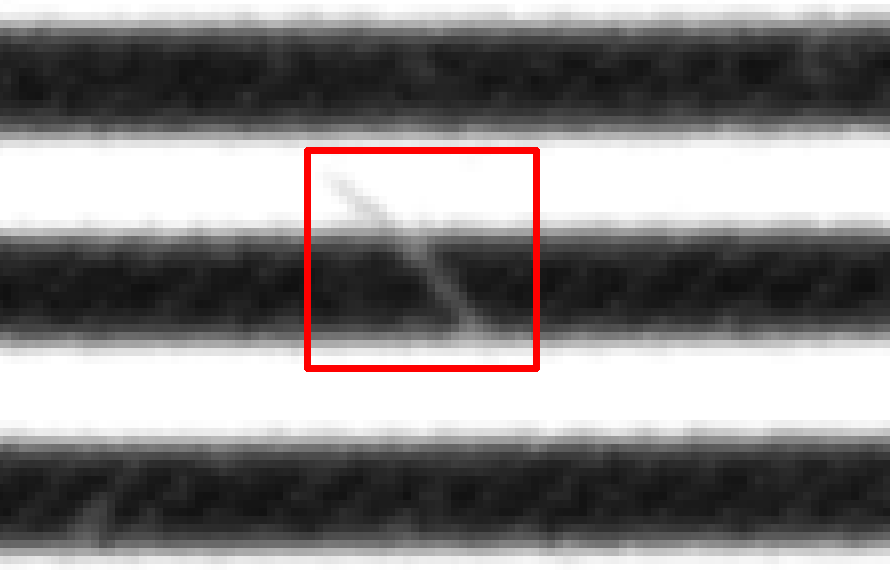
\includegraphics[width=0.5\textwidth]{01_einfuehrung/deflektometrie/qualitativeSichtpruefung/figures/scratch}
	\caption[Kratzer an Hell-Dunkel-Übergang eines Streifenmusters]{Kratzer an Hell-Dunkel-Übergang eines Streifenmusters}
	\label{img:scratch}
\end{figure}

%\noindent
%Dieser Ansatz zum Detektieren von Kratzern und ähnlichen Defekten wird im Kapitel \ref{sec:prototyp} weiter erläutert.

\noindent
Durch die Variabilität der Deflektometrie und der offenen Definition der qualitativen Sichtprüfung lassen sich z. B. durch Veränderung des Musters zahlreiche verschiedenste Verfahren aufstellen, um eine Objektoberfläche zu analysieren.
Aus dem Grund kann keine allgemeine Funktionsweise von deflektometrischen Verfahren für die qualitative Sichtprüfung beschrieben werden.
%Stattdessen wird im Rahmen dieses Projekts auf ein bestimmtes ausgewähltes Verfahren genauer eingegangen, dass für die konkreten Anwendungsfälle aus Kapitel \ref{sec:projektthema} Ergebnisse liefern konnte.
}
}
